% !TEX root = ../gnss_interference_resistant_thesis.tex
\documentclass[main.tex]{subfiles}

\begin{document}

\subsection{HackRF laikinės sinchronizacijos matavimas}\label{sec:time_sync}

Tikrinant laikinę sinchronizaciją, naudojamas stendas, kurio
blokinė diagrama pavaizduota \ref{fig:measurement_stand}~pav.
Kaip signalo šaltinis naudojamas HackRF One siųstuvo konfigūracijoje,
jo siunčiamas signalas yra gauso triukšmas.

\begin{figure}[h]
    \begin{centering}
    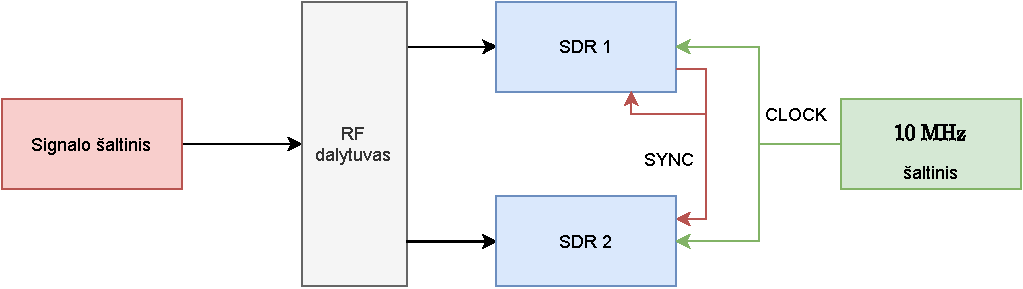
\includegraphics[scale=0.9]{drawings/measurement_stand}
    \par\end{centering}
    \protect\caption{\label{fig:measurement_stand}Matavimo stendo schema.}
\end{figure}

Matavimui naudojami 2 HackRF One radijai, sukonfigūruoti imtuvo konfigūracijoje.
Tarp jų yra sujungtas sinchronizacijos signalas kaip aprašyta \ref{sec:beamforming_concept}
skyriuje, bei naudojamas bendras $10\ \mathrm{MHz}$ šaltinis.

Turint IQ taškus iš abiejų imtuvų, norint rasti signalo užlaikymą tarp imtuvų, galime
pasinaudoti koreliacijos operacija, kurios rezultatas bus užlaikymas tarp signalų.
Tarkime, kad pirmojo imtuvo taškai yra seka $x[n]$, o antrojo $y[n]$. Kryžminė
koreliacija $r_{xy}$ apibrėžiama:

\begin{equation}
    r_{xy}[l] = \sum_{n=-\infty}^\infty x[n]y[n-l],\quad l=0,\pm 1, \pm 2,...\ .
    \label{eq:corelation}
\end{equation}

\noindent Pritaikę \refeq{eq:corelation} lygtį, gauname koreliacijos rezultatą, kurio
maksimumas nurodo uždelsimą tarp dviejų signalų.

\begin{figure}[h]
    \begin{centering}
    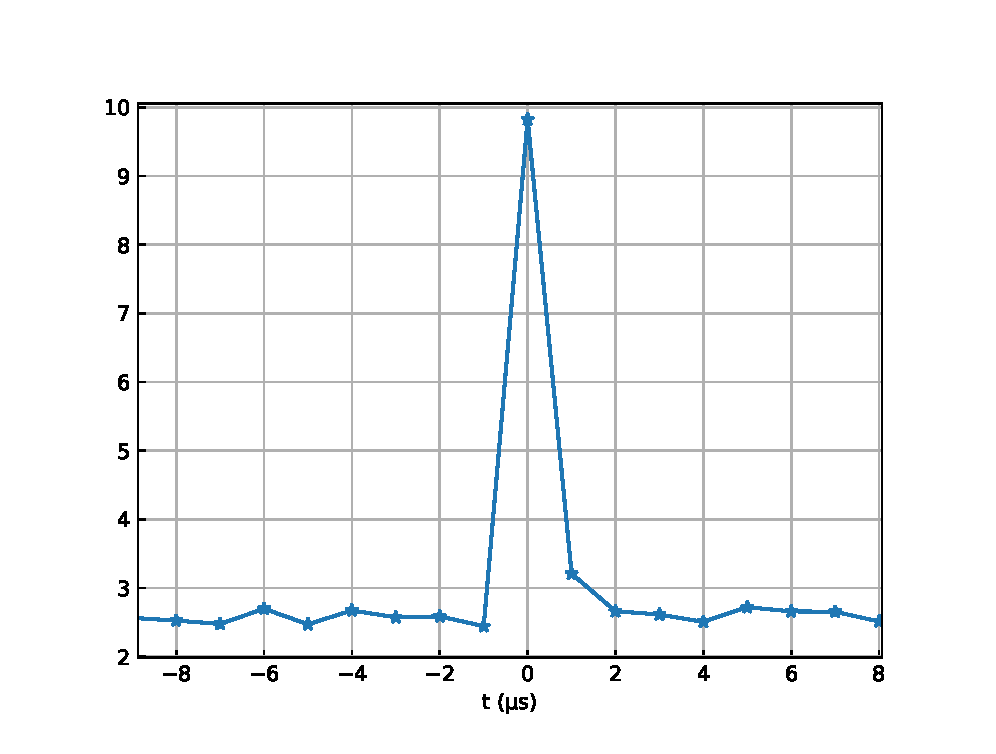
\includegraphics[scale=1.0]{drawings/time_sync}
    \par\end{centering}
    \protect\caption{\label{fig:time_sync_result}HackRF signalų koreliacijos rezultatas.}
\end{figure}

\ref{fig:time_sync_result}~pav. galime matyti, kad koreliacijos maksimumas yra centruotas
ties $0\ \mathrm{\mu s}$, todėl galime daryti išvadą, kad imtuvai yra sinchronizuoti laike,
$\pm 1$ taško tikslumu (kai skaitymo dažnis yra $f_s=2\ \mathrm{MHz}$).
Rezultatas sutampa su rezultatais pateiktais \cite{hackrf_sync} straipsnyje.

\subsubsection{Koreliacijos skaičiavimo optimizavimas}

\ref{sec:time_sync} skyriuje aprašytas algoritmas reikalauja didelių skaičiavimo pajėgumų,
todėl taikyti šio algoritmo realiu laiku neišeina. Algoritmas gali būti optimizuotas
pasinaudojus koreliacijos savybe, kuri lemia tai, kad sudauginus kompleksiškai jungtines signalų
Furje transformacijas, gauname koreliacijos Furje transformaciją. Rezultatui pritaikius
atvirkštinę Furje transformaciją gauname koreliacijos rezultatą.
Sparčiam Furje skaičiavimui naudosime FFT (angl. Fast Fourier transform) algoritmą, kuris
tinkamas naudoti su diskretizuotu signalu.

Algoritmo eiliškumas:
\begin{enumerate}
    \item Atliekame abiejų signalų Furje transformacijas pasinaudojus FFT algoritmu;
    \item Sudauginame vieną signalą su kito kompleksinio jungtinu rezultatu;
    \item Atliekame atvirkštinę Furje transformaciją pasinaudojus FFT algoritmu;
\end{enumerate}

\end{document}
